%%
%% Hochschule Emden-Leer --  Abschlussarbeit
%%
%% Hauptdokument
%%
%% 23.01.09 Tschirley V.01
%% 24.08.14 Bergen V.03
%% 28.11.14 Lorenz V.04
%%
%%%%%%%%%%%%%%%%%%%%%%%%%%%%%%%%%%%%%%%%%%%%%%%%%%%%%%%%%%%%%%%%%%%%%
\documentclass[11pt, a4paper]{book}
\usepackage[hang]{footmisc}
\setlength\footnotemargin{10pt}

%% Übersetzen als Entwurf
%\usepackage[entwurf]{latexTemplate/bhtThesis}
%% Übersetzen für die Abgabe
\usepackage[abgabe]{latexTemplate/bhtThesis}	
\typeout{Master-Thesis Sascha Lorenz Hochschule Emden-Leer V0.1}
\usepackage{blindtext}   %für Blindtext, warum auch immer; ohne geht maketitle nicht: EB, 01.05.2014
\usepackage{listings}
\lstset{ 
  literate={ö}{{\"o}}1
           {ä}{{\"a}}1
           {ü}{{\"u}}1
           {Ö}{{\"O}}1
           {Ä}{{\"A}}1
           {Ü}{{\"U}}1
           {ß}{{\ss}}2
}

% Symbole
\usepackage{trsym} % http://ftp.gwdg.de/pub/ctan/fonts/trsym/trsym.pdf
\usepackage{bytefield} %http://ftp.uni-erlangen.de/mirrors/CTAN/macros/latex/contrib/bytefield/bf-example.pdf
\usepackage{bibgerm}
\usepackage{MnSymbol}
\usepackage{lmodern}
\usepackage{multibib}
%\usepackage[acronyms]{glossaries}
\usepackage[acronym,style=long,toc=true,numberedsection=autolabel]{glossaries} 
%\robustify{\gls}

\usepackage{booktabs}
\makeglossaries


\newcites{lit}{Literaturverzeichnis}
\newcites{int}{Internetquellen}

\usepackage{listings,xcolor}

\definecolor{listingBackground}{rgb}{0.97,0.97,0.97}
\definecolor{stringColor}{rgb}{0.37,0.37,0.37}
\lstset{
	basicstyle=\footnotesize\ttfamily,
	numbers=left,
	numberstyle=\tiny,
	%stepnumber=2,
	numbersep=5pt,
	tabsize=2,
	extendedchars=true,
	breaklines=true,
	keywordstyle=\color{red},
	frame=b,
	stringstyle=\color{stringColor}\ttfamily,
	showspaces=false,
	showtabs=false,
	xleftmargin=17pt,
	framexleftmargin=17pt,
	framexrightmargin=5pt,
	framexbottommargin=4pt,
	backgroundcolor=\color{listingBackground},
	showstringspaces=false
}

\usepackage{caption}
\DeclareCaptionFont{white}{\color{black}}
\DeclareCaptionFormat{listing}{\colorbox[rgb]{0.87, 0.87, 0.87}{\parbox{\textwidth}{\hspace{15pt}#1#2#3}}}
\captionsetup[lstlisting]{format=listing,labelfont=white,textfont=white,singlelinecheck=false,margin=0pt,font={bf,footnotesize}}

\usepackage[babel,german=quotes]{csquotes}


\DeclareQuoteStyle{fquotes}
  {\em}{}{\em}{}

\newcommand*{\myfquote}[1]{%
  \begingroup%
    \setquotestyle{fquotes}%
    \enquote{#1}%
  \endgroup%
}

\newif\ifmyblockquote
\newcommand*{\myblockquote}{%
\myblockquotetrue\blockquote}

\DeclareQuoteStyle[italics]{german}
[\itshape]
[\itshape]
{\quotedblbase}
{\textquotedblleft}
[0.025em]
{\quotesinglbase}
{\fixligatures\textquoteleft}
\DeclareQuoteAlias[italics]{german}{german}


\renewcommand\mkblockquote[4]{\enquote{#1#2#3}#4}

\providecommand{\e}[1]{\ensuremath{\times 10^{#1}}}

%%
%% Pfad zu den Bildern
%%
\graphicspath{
  {pictures/},
  %{einleitung/pictures},
  %{kapitel1/pictures/},
  %{kapitel2/pictures/}
}

%\usepackage{pgfplots}
%\usepgfplotslibrary{dateplot}



%%
%% Einbinden persönlicher macros 
%%
\input{personalMacros.tex}

%% Message
\typeout{-----------------------------------------------------------}
\typeout{----> thesis.tex ---- Zentrales Dokument-------------------}
\typeout{-----------------------------------------------------------}

\version{1.56}
\abgabedatum{{07}. {März} {2015}}
%%
%% Titel, Autor und Betreuer
%%
\fachbereich{Technik} 
\studiengang{Medieninformatik-Online (Master)}
\autor{Sascha P. Lorenz}
\matrnr{501 63 21}
\titel{Big Data Processing mit Apache Spark}
\untertitel{}
\betreuerFeld{
  \begin{tabular}{llr}
    
    \textbf{1. Betreuer} & Herr~Prof.~Dr.~Edlich & Beuth Hochschule für Technik\\
    \textbf{2. Betreuer} & Herr~Prof.~Dr. Schiemann-Lillie & Hochschule Emden-Leer
  \end{tabular}
}

%%\renewcommand{\baselinestretch}{1.05} 
\renewcommand{\arraystretch}{1.3}
\pagenumbering{Alph}
\begin{document}
\pagestyle{fancy}
\newacronym{glo:mpeg}{MPEG}{Motion Pictures Expert Group}


\cleardoublepage

\input{titelseiten.tex}
\frontmatter



\mainmatter

\pagenumbering{arabic}
%%%%%%%%%%%%%%%%%%%%%%%%%%%%%%%%%%%%%%%%%%%%%%%%%%%%%%%%%%%%%%%
%% Die Kapitel der Arbeit

\chapter{Einführung}
\label{chapter:einfuehrung}

``Big Data" ist insbesondere in den letzten Jahren immer stärker in den verschiedensten Zusammenhängen in den allgemeinen Sprachgebrauch vorgedrungen und ist hier einem ständigen Bedeutungswandel ausgesetzt. Besonders in letzter Zeit wird dieses Thema auch verstärkt kontrovers diskutiert.  

Im ersten Kapitel soll der Begriff „Big Data“ jenseits von Management-Hype und Skepsis rational definiert werden. Des Weiteren werden einige grundlegende Konzepte des Umgangs mit sehr großen und unstrukturierten Datensätzen diskutiert und im Speziellen die Motivation hinter den Apache Frameworks Hadoop und Spark vorgestellt.  

Das zweite Kapitel beschäftigt sich mit dem Berkeley Data Analytics Stack (BDAS), mit dem von der UCLA Berkeley rund um Hadoop ein leistungsfähiger Infrastruktur-Stack für die Einsatzbereiche von Big Data Analytics geschaffen wurde. 

Innerhalb vom BDAS etabliert sich langsam auch eine schnellere und flexiblere Alternative zu Hadoop: Apache Spark. Im dritten Kapitel wird diese neue Kerntechnologie vorgestellt, die zugleich auch den Hauptteil dieses Wissenschaftlichen Projektes darstellt. 

Im vierten Teil dieser Ausarbeitung wird Spark in der praktischen Anwendung gezeigt inklusive Installation und ersten kleineren Beispielen sowohl direkt in Spark, als auch aus darüber liegenden Schichten aus dem Stack. 

\section{Was versteht man unter ``Big Data“?}
\label{section:was versteht man unter ``Big Data”?}


Der Begriff ``Big Data“ wurde vermutlich zum ersten Mal Ende des 20. Jahrhunderts von John R. Marshey, damals Chefwissenschaftler bei Silicon Graphics, im Rahmen einer Usenix-Konferenz öffentlich erwähnt \citeint{jt11}. Mittlerweile ziert dieser Begriff gefühlt jedes zweite Cover von IT-Zeitschriften mit Business-Fokus und auch Manager und ``Sales-Professionals“ werten Ihre Produktpräsentationen gerne mit diesem Buzzword auf.  Aber dieser Begriff ist nicht nur positiv assoziiert. Besonders seit Bekanntwerden der Tätigkeiten des Amerikanischen Auslandsgeheimdienstes weckt die Vorstellung des „Datensammelns“ in großen Dimensionen auch Misstrauen. 

	Im Rahmen dieser Arbeit soll jedoch ausschließlich die technische Betrachtung und die exemplarische Darstellung von möglichen Anwendungsgebieten diskutiert werden.




Wie lässt sich der Begriff „Big Data“ abgrenzen? Es existiert keine abschließend eindeutige Definition, jedoch gibt es einige Attribute, die sich in einem Großteil der Fachliteratur etabliert haben. Der Artikel aus dem O'Reilly Radar zum Thema \citeint{dumbhill} fasst dies folgendermaßen zusammen: 

\enquote{Big data is data that exceeds the processing capacity of conventional database systems. The data is too big, moves too fast, or doesn’t fit the structures of your database architectures.}

Neben der reinen Menge spielt also offensichtlich auch die mangelnde oder fehlende Strukturierung und unter Umständen die Flüchtigkeit der Daten eine nicht unerhebliche Rolle. Dies können beispielsweise Daten aus Social-Media-Quellen sein, die aus allen möglichen verschiedenen Einzeldaten bestehen, Daten von Sensoren, die permanent überwacht werden müssen, oder Datenströme (Video, Audio, Bilder, Text), die nach einheitlichen Kriterien gefiltert werden sollen, um hier nur einige Beispiele zu nennen. Auch die temporäre Komponente ist ein Einsatzgebiet für „Big Data“, und auch hier ist wieder das Beispiel der Datenströme heranzuziehen. 

Bei der Definition von Big Data werden laut des BITKOM-Ratgebers zum Thema „Big Data“ \citeint{bk14} auch immer wieder die „Three Vs“ angeführt. Dies sind Volume, also die Datenmenge, Variety, die Datenvielfalt und Velocity, die Geschwindigkeit der Auswertung. 

Die sinnvolle Analyse dieser Daten kann Unternehmen oder anderen Organisationen wichtige Informationen z.B. über Marktentwicklungen, bestimmte Kundenbedürfnisse, Epedemie-Ausbreitungen oder andere wichtige Sachverhalte liefern. Diese Analyse inklusive der dazu verwendeten Werkzeuge wird allgemein „Big Data Analytics“ genannt. 

\section{Ansätze für ``Big Data Analytics“}
\label{section:ansaetze für ``Big Data Analytics“}


``Big Data Analytics“ umfasst Methoden und Werkzeuge zur automatisierten oder interaktiven Erkennung und daraufhin auch Verwendung von bestimmten Mustern und Assoziationen. Dies sind unter anderem:

\begin{itemize}
		\item Prediction-Models zur Vorhersage bestimmter Sachverhalte
		\item statistische Verfahren, wie beispielsweise Logistic Regression oder k-means-Algorithmen 
		\item Optimierungs- und Filteralgorithmen 
		\item Werkzeuge zum Datamining
		\item Textanalyse
		\item Bild- und Tonanalyse
		\item Datenstromanalysen
\end{itemize}	



Nach dem BITKOM-Leitfaden [BK14] besteht die Taxonomie der Big-Data-Technologien grundsätzlich aus vier Schichten:


\begin{itemize}
		\item Daten-Haltung
		\item Daten-Zugriff 
		\item Analytische Verarbeitung
		\item Visualisierung
\end{itemize}	


Diese werden durch Daten-Integration und Daten-Governance, sowie Daten-Sicherheit flankiert, um den Weg von Rohdaten bis zu nutzbaren Erkenntnissen in existierende Standards einzubetten.

Zahlreiche Hersteller herkömmlicher relationaler Datenbanksysteme versuchen derzeit, ihre bestehenden Lösungen mit dem Label „Big Data“ zu versehen und diese so weiterhin in diesen sich verändernden Marktsegmenten zu positionieren. Wenn „Big Data“ jedoch jenseits der Datengröße definiert wird und auch unstrukturierte und temporäre Daten-Stacks oder –ströme zu verarbeiten oder zu analysieren sind, stoßen RDBMS sehr schnell an ihre Grenzen. Doch auch was die Skalierbarkeit angeht, sind relationale Datenbanken meist nicht hinreichend flexibel \citeint{ml10}. 

Für die Anforderungen an dedizierte Aufgaben im Bereich Big-Data-Analytics sind seit einigen Jahren einige Frameworks auf dem Markt, die in allen drei oben genannten Aspekten besser geeignet sind, als RDBMS. Der Ansatz ist hier primär, die Verarbeitung zu dezentralisieren, also auf unabhängige Knoten in einem Rechner-Cluster zu verteilen und nur Referenzen auf die Clusterknoten zentral zu verwalten.  

Es existieren mittlerweile Lösungen am Markt, die speziell diese Aufgaben für derartige Aufgaben entwickelt wurden. Hier wären unter anderem Hadoop, Spark, HPCC, GPMR, Mincmeat, Sphere, Bashreduce und R3 zu nennen. Bis auf HPCC setzen alle eben genannten Implementierungen generell oder in Teilen auf das Programmiermodell MapReduce. 

Der zweifellose De-facto-Standard in diesen Bereichen ist bereits seit einiger Zeit das Open-Source-Framework Apache Hadoop. Auf Hadoop basierend existieren etliche Derivate. Unter anderem sind hier Cloudera, Amazon Elastic MapReduce, Apache BigTop, Datameer, Apache Mahout, MapR und IBM PureData System zu nennen. 



	





\section{Motivation für Apache Hadoop/Spark}
\label{section:motivation für Apache Hadoop/Spark}

Anfang des 21. Jahrhunderts wurde das Bedürfnis für Möglichkeiten, sehr große Datenmengen effizient verarbeiten zu können, stetig größer. Nicht zuletzt durch die zu dieser Zeit exponentiell steigende Menge von Inhalten im World Wide Web und deren Indexierung durch Suchmaschinen wie Google. Davon motiviert wurde 2002 das Projekt „Nutch“ mit dem Ziel gestartet, ein geeignetes Such- und Crawlersystem frei verfügbar zu machen. Die ersten Versuche skalierten sehr schlecht, bis Google 2003 die Funktionsweise ihres verteilten Dateisystem GFS (Google File System) veröffentlichte. Somit konnten die sehr großen Dateien, die durch die Indexierung entstanden, effizient auf verschiedene Knoten verteilt gespeichert werden und die Verwaltung dieser Knoten und Dateien aus dem eigentlichen Indexierungs- und Suchprozess ausgelagert werden. 

Im Jahre 2004 publizierte Google den MapReduce-Algorithmus, der unter anderem die Indexierungs- und Analysefunktionen parallelisieren, delegieren und sinnvoll bündeln kann. In Nutch wurden daraufhin sämtliche wichtige Algorithmen auf MapReduce umgestellt, nachdem zuvor auch GFS unter dem Namen NDFS (Nutch Distributed File System) integriert wurde. Die möglichen Anwendungsgebiete von Nutch waren damit auch weit über das reine Suchen und Indexieren von Webseiten hinaus gewachsen. 2006 wurde aus Nutch ein Unterprojekt mit dem Namen Hadoop ausgegliedert, das im Jahre 2008 zum Apache Top-Level-Project ernannt wurde. Zu dieser Zeit nutzten bereits Firmen wie Yahoo!, Facebook oder die New York Times Hadoop. Ein exemplarischer Anwendungsfall bei der NY Times war, mit Hilfe der Hadoop-basierten EC2-Cloud von Amazon ca. vier Terabyte gescannter Archivdateien in PDF-Dateien umzuwandeln und dies in weniger als 24 Stunden auf 100 Knoten. Auch beim Sortieren von sehr großen Datenmengen stellten Hadoop-basierte Systeme nach und nach sämtliche Rekorde ein [TW09]. 

Hadoop und Hadoop-basierte System gelten mittlerweile als Industriestandard für Big-Data-Analytics-Anwendungen. Jedoch ist Hadoop nicht für alle Anwendungsgebiete gleichermaßen geeignet. Aufgrund der Charakterisierung der Paradigmen für Big Data Analytics im Paper „Frontiers in Massive Data Analysis“ der National Academic Press [NRC13], lassen sich die Einsatzgebiete und Schwächen für Hadoop ermitteln [VA14].

So lassen sich mit Hadoop einfachere statistische Aufgabenstellungen sehr gut umsetzen. Dazu gehören Mittelwert, Median, Varianz und allgemein abzählende sowie ordnende Statistikaufgaben. Dies sind in der Regel Anwendungen mit einer Laufzeitkomplexität von O(n) für n Betrachtungswerte. Sie sind meist auch sehr gut parallelisierbar und somit sehr gut für Hadoop geeignet.    



Für linear-algebraische Berechnungen (lineare Regression, Eigenwertproblem, Hauptkomponentenanalyse), generalisierte n-Körper-Probleme (mit einer Komplexität 
von O(n²) oder O(n³)), Graphentheorie, Optimierungsprobleme (Verlust-, Kosten- oder Energiefunktionen, sowie  Integrations- und Ausrichtungsfunktionen ist Hadoop nur in jeweils einfacher Problemausprägung einsetzbar. Auch für Interaktive Abfragen ist Hadoop nur bedingt geeignet, da es ursprünglich für die Batch-Verarbeitung entwickelt wurde.

Aus diesem Grund wurde am AMPLab der University of California in Berkeley nach Alternativen geforscht, die auch für komplexe linear-algebraische Probleme, generalisierte n-Körper-Probleme und diverse Optimierungsprobleme geeignet sind. Das Ergebnis ist Spark, mittlerweile Apache Top-Level-Projekt und dazu geeignet, die Nachfolge von Hadoop als Big-Data-Analytics-Framework anzutreten. 

\section{Ziel und Aufbau dieser Arbeit}
\label{section:ziel dieser Arbeit}

Die vorliegende Arbeit beschäftigt sich mit Apache Spark und dem dazugehörigen Ökosystem bestehend aus Schichten  mit verschiedenen Bibliotheken, dem Berkeley Data Anaytics Stack (BDAS). Auf dem Markt befindet sich bislang noch verhältnismäßig wenig Literatur zu diesem Thema und wenn, dann werden zumeist Teilaspekte für bestimmte Anwendungsbereiche gekapselt betrachtet. Diese Arbeit soll zunächst einen ganzheitlichen Überblick über den Stack bieten. Hier werden die einzelnen Schichten des Stacks kurz beschrieben und gegebenenfalls Alternativlösungen zu den jeweiligen Implementierungen vorgestellt. 

Insbesondere werden in den darauffolgenden Kapiteln die Statistik- und Vorhersagebibliotheken MLLib im Gegensatz zu H2O betrachtet und die Kernimplementierung von Spark mit dem neueren Framework Apache Flink verglichen. Die Bibliotheken des Caching-Frameworks Tachyon werden vorgestellt, sowie die Streaming-Bibliothek Spark Streaming und die Graphenanwendung GraphX. 

Dann werden jeweils praktische Anwendungsbeispiele gezeigt und im Zuge dessen die APIs von Spark und MLlib insbesondere vorgestellt.   



\chapter{Grundlagen von Spark}
\label{chapter:grundlagen von Spark}


Rund um Hadoop beziehungsweise Spark wurde in Berkeley ein ganzer Infrastruktur-Stack für Big-Data-Analytics aufgebaut, der BDAS.


\section{Der Berkeley Data Analytics Stack (BDAS)}
\label{section:der Berkeley Data Analytics Stack (BDAS)}

	
	Im Folgenden wird der Big Data Analytics Stack (BDAS) näher vorgestellt, der wie in der Einführung bereits erwähnt um Hadoop, bzw. Spark als Hauptbestandteile herum aufgebaut ist. Der BDAS wurde von den AMPLabs (kurz für „algorithms, machines and people“) von der University of California in Berkeley aufgrund von Forschungs-ergebnissen im Bereich der Analyse sehr großer Datenmengen ins Leben gerufen. 

Der Einsatz des BDAS kann laut Vijay Agneeswaran [VA14] dabei helfen, unter anderem Fragen wie die folgenden zu beantworten: 

\begin{itemize}
		\item Wie segmentiert man am besten eine Menge von Nutzern und kann herausfinden, welche Nutzersegmente an bestimmten Kampagnen interessiert sein könnten?
		\item Wie kann man richtige Metriken für Nutzer-Engagement in Social-Media-Applikationen herausfinden?
		\item Wie kann ein Video-Streaming-Dienst für jeden Nutzer dynamisch ein optimales Content-Delivery-Network (CDN) basierend auf Daten wie Bandbreite, Auslastung, Pufferrate, etc Auswählen?
		
\end{itemize}	


Prinzipiell sind die in der Einführung in Kürze beschriebenen Einschränkungen von Hadoop und die damit verbundene Motivation für Spark auch die Motivation für den BDAS. 


In Abbildung 2.1 wird eine Übersicht über die drei Hauptschichten des BDAS gezeigt. Rot dargestellt ist hier jeweils die von den AMPLabs empfohlene Implementierung.

\begin{figure}[htb!]
\centering
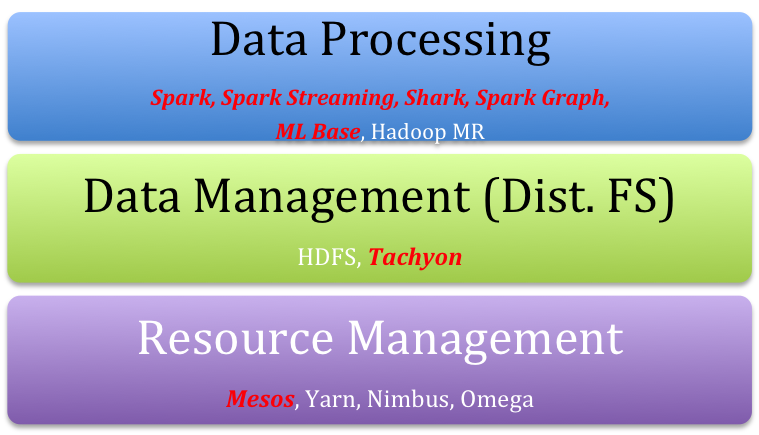
\includegraphics[width=1.0\textwidth]{bilder/2_1_stack.png}
\caption{Grobübersicht über den BDAS mit den drei Hauptschichten}
\label{fig:grobübersicht über den BDAS mit den drei Hauptschichten}
\end{figure}
 


In Abbildung 2.2 ist der Aufbau des BDAS nochmals schematisch dargestellt. Die grün hinterlegten Elemente markieren die Bestandteile des aktuellen BDAS, die violett hinterlegten zeigen alternative Implementierungen auf der jeweiligen Schicht. Grün schraffiert ist die Applikationsschicht, wo Applikationen oberhalb von Spark und den direkten Anwendungen angesiedelt sind. 

\begin{figure}[htb!]
\centering
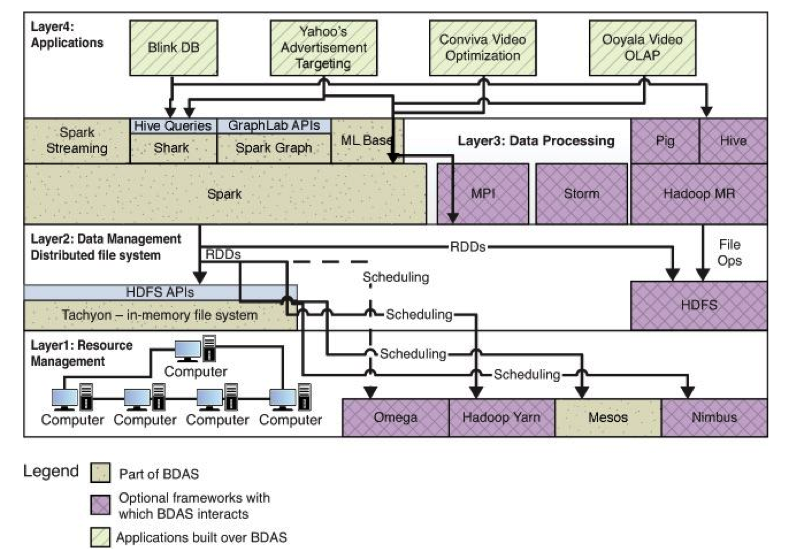
\includegraphics[width=1.0\textwidth]{bilder/2_2_stack.png}
\caption{Der BDAS. Abbildung aus „Big Data Analytics Beyond Hadoop“, S 15 \protect\citelit{va14}}
\label{fig:bdas]}
\end{figure} 


\section{Apache Mesos}
\label{section:apache Mesos}


Bei Apache Mesos handelt es sich um ein Cluster-Management-Framework für Anwendungen, die in verteilten Serverpools laufen sollen. Bestandteil von Mesos ist wiederum Apache ZooKeeper, das für Konfigurationsinformationen, Naming-Services und die Synchronisation von verteilten Anwendungen zuständig ist.  

Mesos wird im BDAS eingesetzt, um die Prozesse von Hadoop/Spark effizient auf die einzelnen Knoten im Cluster zu verteilen. Besonders das Ressourcen-Management und –Monitoring innerhalb des Clusters ist ein wichtiger Faktor, um Jobs performant auf verteilten Systemen ausführen zu können. Auch das Fehlerhandling für Knoten, Prozesse und im Netzwerk wird im Berkeley-Stack von Mesos übernommen. 

Ein besonderer Vorteil von Mesos gegenüber Yarn oder anderen Alternativen, wie dem Cloudera Cluster Manager oder Ambari von Hortonworks ist die Möglichkeit, verschiedene Frameworks gleichzeitig und isoliert in einem Cluster betreiben zu können. So kann beispielsweise Hadoop mit Spark in einer gemeinsamen Infrastruktur koexistieren.   
	
\section{Hadoop Distributed File System (HDFS) und Tachyon}
\label{section:hadoop Distributed File System (HDFS) und Tachyon}


Das Hadoop Distributed File System basiert ideologisch auf dem GoogleFileSystem (GFS) und hat zum Zweck, zuverlässig und fehlertolerant sehr große Dateien über verschiedene Maschinen hinweg in verteilten Umgebungen zu speichern. In entsprechenden Veröffentlichungen von Hortonworks \citeint{ho14} wird von Produktivsystemen berichtet, die bis zu 200 PetaByte an Datenvolumen in einem Cluster von 4500 Servern basierend auf HDFS verwalten.

HDFS wurde speziell für den Einsatz mit MapReduce entwickelt, ist also auf geringe Datenbewegungen ausgelegt, da MR die Berechnungsprozesse jeweils zu den physischen Datensätzen selbst bringt und nicht, wie herkömmlich, die Daten zu den Prozessen geliefert werden müssen. So wird massiv Netzwerkverkehr innerhalb des Clusters eingespart und letztlich werden nur Prozesse und Prozessergebnisse verschickt.  

Die Hauptbestandteile von HDFS sind der sogenannte NameNode, der die Metadaten des Clusters verwaltet und die DataNodes, die die eigentlichen Daten halten. Dateien und Verzeichnisse werden vom NameNode durch inodes repräsentiert. Diese wiederum enthalten Informationen über Zugriffsrechte, Zugriffszeiten oder Größenangaben der Dateien.



\begin{figure}[htb!] 
\centering
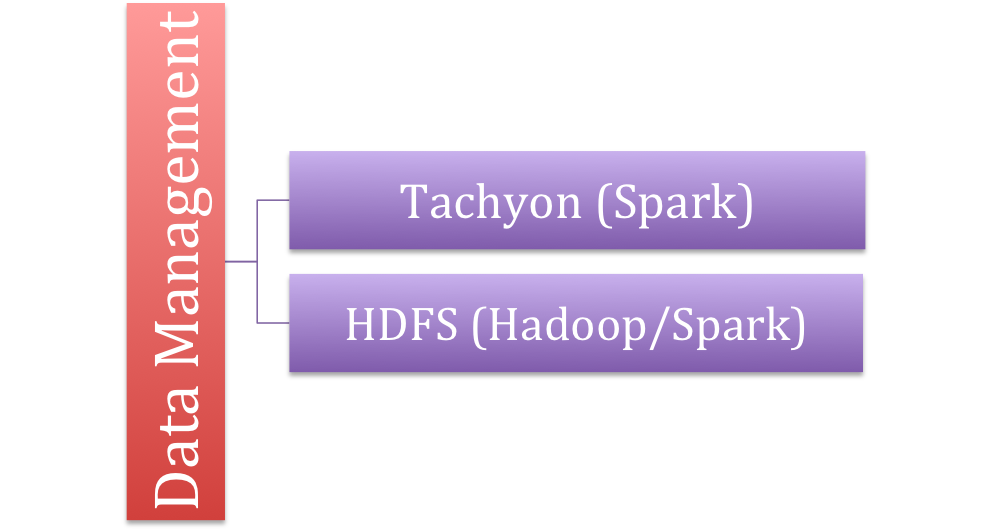
\includegraphics[width=1.0\textwidth]{bilder/2_3_stack.png}
\caption{Der Datamanagement-Layer im BDAS mit HDFS und Tachyon}
\label{fig:datamgmtlayer}
\end{figure} 

 

In Abbildung 2.3 wird die Datenmanagementschicht des BDAS nochmals detaillierter dargestellt. Hier ist erkennbar, dass reine Hadoop-Implementierungen direkt auf dem HDFS aufsetzen, da das HDFS für MapReduce optimiert ist. 

Kommt hingegen Spark zum Einsatz, lässt sich wahlweise direkt das HDFS ansprechen oder alternativ eine Zwischenschicht nutzen, die auf das In-Memory-Modell von Spark zugeschnitten ist. Dies ist innerhalb des BDAS das verteilte Dateisystem Tachyon. Hier werden die zu verarbeitenden oder zu analysierenden Datensätze direkt in den Hauptspeicher des jeweiligen Knoten gecached. Somit werden Lade- und Speicheroperationen auf Massenspeicher minimiert und eine massiv höhere Ausführungsgeschwindigkeit erreicht. Unterhalb von Tachyon ist nach wie vor ein HDFS für die persistente Datenhaltung notwendig. Alternativ kann auch das Amazon S3-File-Sytem eingesetzt werden. Tachyon wurde direkt innerhalb der AMPLabs entwickelt und ist mittlerweile fester Bestandteil des BDAS.  


\section{Apache Spark}
\label{section:apache Spark}

Spark ist das Herzstück des BDAS. Bei Spark handelt es sich um ein open-source Data-Analytics-Framework, das, wie Hadoop, speziell für die Bedürfnisse im Rechner-Cluster konzipiert ist. Auch Spark nutzt das HDFS entweder direkt, oder indirekt über Tachyon. Im Gegensatz zu Hadoop bietet Spark jedoch Funktionen für In-Memory-Cluster-Berechnungen und ist nicht zwingend an MapReduce gebunden. Besonders interaktive Analyse oder Verarbeitung der Daten, Abfragen über verteilte Dateien und iterative 

Lernalgorithmen erfahren so laut AMPLab eine bis zu hundertfache Ausführungs-geschwindigkeit im Gegensatz zu Hadoop. Auch die im ersten Kapitel angesprochenen Schwächen von Hadoop bei Berechnungen von komplexen linear-algebraischen Problemen, generalisierten n-Körper-Problemen, diversen Optimierungsproblemen und diversen anderen Aufgaben, treten bei Spark auf Grund der offenen Architektur und der Zerlegung von Datensätzen in die sogenannten Resilient Distributed Datasets (RDD) nicht mehr auf.

Spark wurde komplett in Scala entwickelt und bietet APIs für Scala, Java (inklusive Lambda-Expressions von Java 8) und Python. Im Labor existieren bereits Spark-Installationen mit bis zu 2000 Knoten, in Produktivsystemen sind bisher Systeme mit bis zu 1000 Knoten im Einsatz \citeint{cm13}. Durch die Möglichkeit, die Datensätze im Speicher für interaktive Analyseaufgaben zu cachen und iterativ abzufragen, ist eine direkte Kommandozeileninteraktion über das integrierte Scala REPL (alternativ auch in Python) möglich. 

Für Spark existieren dedizierte Bibliotheken für Verarbeitung von Datenströmen, Machine-Learning und Graphenverarbeitung. Ähnliche Artefakte existieren auch für Hadoop (Mahout, Vowpal Wabbit, etc.), jedoch ist die Architektur von Spark wesentlich besser für derartige Anwendungsbereiche zugeschnitten. 
   
\subsection{Spark Streaming}
\label{section:spark Streaming}


Spark Streaming ist eine der oben genannten Bibliotheken, die Spark um dedizierte Anwendungsbereich erweitert. Hierbei handelt es sich um eine Erweiterung, um die integrierte API von Spark für Anwendungen auf Datenströmen nutzen zu können. Das Programmiermodell unterscheidet nicht zwischen Batch- und Streaming-Anwendungen. So lassen sich beispielsweise Datenströme zur Laufzeit mit Archivdaten vergleichen und direkt Ad-hoc-Abfragen auf die Ströme formulieren. Im Fehlerfall ermöglicht Streaming zahlreiche Wiederherstellungsoptionen, sowohl von verlorenen Datenströmen, als auch von Einstellungen. Ein Anwendungsbeispiel ist die Echtzeitanalyse von Twitter-Meldungen. 

\subsection{GraphX}
\label{section:graphX}


GraphX ist eine Erweiterung für Spark, die verteilte, flexible Graphen-Anwendungen in einem Spark-Cluster ermöglicht \citeint{xg13}. Besonders in den Disziplinen „Machine Learning“ und „Data Mining“ ist die Anwendung komplexer Graphen unerlässlich. Graph-datenbanken kommen immer dann zum Einsatz, wenn stark vernetzte Informationen und ihre Beziehungen zueinander interessant sind. Hier werden die Entitäten als Knoten behandelt, die Beziehungsart definiert die Kanten. Die Kanten können auch gewichtet 

sein. Ein konkretes Beispiel sind die Mitglieder eines sozialen Netzwerks mit ihrem jeweiligen Beziehungsgeflecht. Je nach Kontaktintensität können diese Beziehungen auch priorisiert werden, was hier dem Kantengewicht entspricht.

GraphX nutzt hier die Vorteile der darunterliegenden Spark-Infrastruktur, in dem durch eine tabellarische Anordnung der Datenstrukturen eine massive Parallelisierung möglich ist und auch der Verarbeitung in RDDs voll unterstützt wird. So sind auch interaktive Operationen auf den Graphen jederzeit über REPL möglich. 

\subsection{MLbase/MLLib}
\label{section:mLbase/MLLib}


MLbase ist eine Sammlung von Bibliotheken und Werkzeugen für Machine-Learning-Anwendungen mit Spark. Sie besteht grundsätzlich aus den drei Teilen MLlib, MLI und ML-Optimizer und ist oberhalb der Spark-Installation angesiedelt, wie auf Abbildung 2.4.3. zu erkennen ist. 

\begin{figure}[htb!]
\centering
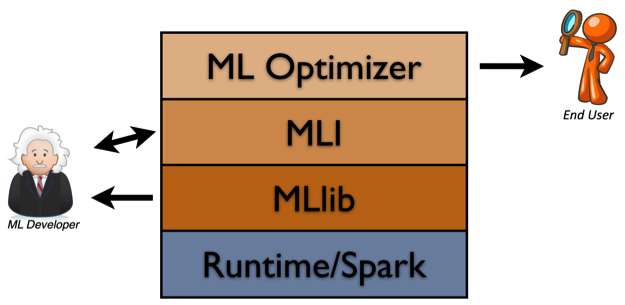
\includegraphics[width=1.0\textwidth]{bilder/2_4_3_mlbase.png}
\caption{Die Bestandteile der MLbase \protect\citeint{ml10}}
\label{fig:mlbase}
\end{figure} 
 


Die MLlib ist eine verteilte Machine-Learning-Bibliothek die für die Spark-Laufzeitumgebung entwickelt wurde und die bekannten Algorithmen für Probleme wie Klassifikation, Regression, Clustering und kollaboratives Filtern enthält.

Bei MLI handelt es sich um eine API, die es ermöglicht, selbst ML-Features zu entwickeln und in erster Linie für komplexere Problemstellungen geeignet ist. Mit MLI lassen sich die Funktionen direkt gegen Spark entwickeln, gegebenenfalls unter Zuhilfenahme der Bibliotheken der MLlib.

Der ML-Optimizer soll ML-Probleme für Endnutzer vereinfachen, in dem Modellauswahlen automatisiert werden. Hierzu werden Features aus der MLlib und der MLI extrahiert und zur Hilfe genommen.



\subsection{Shark}
\label{section:shark}



Hive ist eine SQL-Query-Engine für Hadoop, die sich großer Beliebtheit in der Hadoop-Community erfreut. Shark ist eine Portierung dieser Engine für Spark, um alle Vorteile der In-Memory-Architektur nutzen zu können und ist kompatibel mit sämtlichen Hive-Daten, -Metastores und –Queries. Im Gegensatz zu Hive, das aus Datensätzen zur Laufzeit Java-Objekte generiert, nutzt Shark eine zeilenorientierte Speicherung mittels Arrays primitiver Datentypen und ist somit selbst in einer Hadoop-Infrastruktur im Mittel bis zu fünfmal schneller als Hive. 

Eine Besonderheit von Shark ist neben seinem SQL-Interface die Möglichkeit, auch Machine-Learning-Funktionen als Abfragen formulieren zu können. 

Für die Anwendung von Shark hat sich die Architektur von Spark mit seinen RDDs als sehr vorteilhaft erwiesen, da Abfragen auf Fehlerhaften RDDs nach dem Neuaufbau des entsprechenden Datasets direkt erneut ausgeführt werden können. 

Ein weiterer Unterschied zu Hive ist die sogenannte Partial-DAG-Execution (PDE). Dies bedeutet, dass logische Abfragepläne in Shark aufgrund gesammelter Statistiken zur Laufzeit flexibel erstellt werden im Gegensatz zu Hive oder herkömmlichen relationalen Datenbanksystemen, wo bereits zur Kompilierungszeit starre physische Abfragepläne generiert werden. Besonders die Machine-Learning- und Failover-Funktionen wären mit einer Planerstellung zu Kompilierzeit nicht umsetzbar. 


\section{Alternative Wege innerhalb des BDAS}
\label{section:alternative Wege innerhalb des BDAS}


Wie in den Abbildungen 2.1 und 2.2 ersichtlich, existieren auf jeder Ebene des BDAS auch alternative Implementierungen. Einige davon werden im Folgenden kurz vorgestellt. 


\subsection{Hadoop MR (MapReduce)}
\label{section:hadoop MR (MapReduce)}


Alternativ zu Spark lässt sich im BDAS auch Hadoop als Kernimplementierung für die Datenanalyse oder -verarbeitung im Cluster einsetzen. Dies könnte beispielsweise sinnvoll sein, wenn die Infrastruktur des Clusters über relativ wenig Hauptspeicher verfügt, so dass Spark seinen In-Memory-Vorteil nicht ausspielen kann und die Aufgaben ohnehin den im ersten Kapitel beschriebenen einfachen statistischen Problemen entsprechen. 
 
Hadoop besteht in erster Linie aus dem Hadoop File System (HDFS) und dem MapReduce-Programmiermodell. Dieses wurde von Google speziell entwickelt, um große Datensätze parallel in Clustersystemen verarbeiten und generieren zu können. 

\begin{figure}[htb!]
\centering
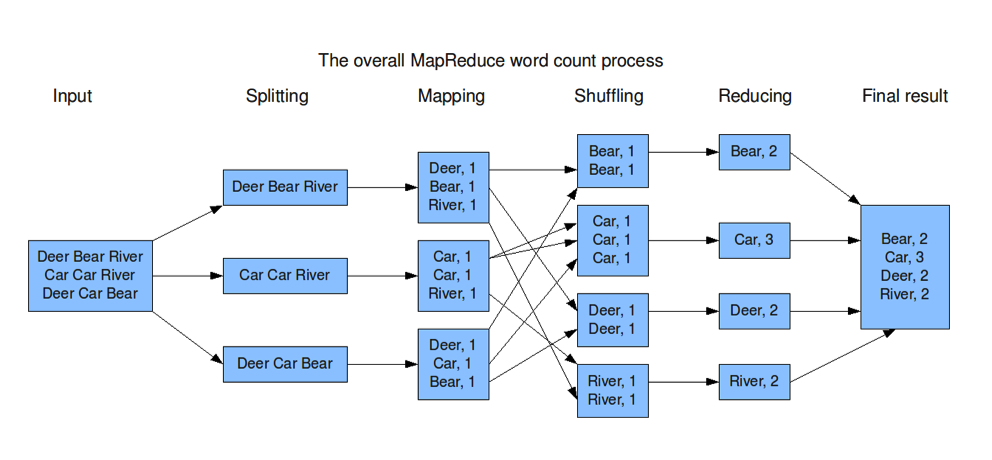
\includegraphics[width=1.0\textwidth]{bilder/2_6_1_wordcount.png}
\caption{Ein konkretes Word-Count-Beispiel für MapReduce  \protect\citeint{xi12}}
\label{fig:wordcount}
\end{figure}   
 


In Abbildung 2.6.1 wird das MapReduce-Modell an einem praktischen Beispiel zur Wortzählung gezeigt. Bei MapReduce wird zunächst eine problemspezifische Map-Funktion definiert. Diese splittet die Ursprungsmenge in gleichgroße Teile, versieht unstrukturierte Worte in einem ersten Schritt mit Standardwerten, um so aus jedem unstrukturierten Datensatz ein Key-Value-Pair zu generieren. Im gezeigten Beispiel wird hier jedem Wert eine Eins als Anzahl zugeordnet. Im nächsten Schritt werden diese so gewonnenen Zwischen-Key-Value-Paare in einem Shuffling-Prozess klassifiziert und die so homogenisierten Pakete auf die Knoten im Cluster verteilt. Nun enthält jede Ausführungseinheit nur noch gleiche Wörter. Im Reduce-Schritt schließlich, werden die gleichartigen Wörter zu Gesamtmengen zusammengefasst, addiert und im Endergebnis aggregiert. 

An dem gezeigten Beispiel lässt sich gut erkennen, dass die einzelnen Ausführungsschritte jeweils parallelisiert und auf separate Knoten im Cluster verteilt werden können. Das Laufzeitsystem kümmert sich um die Details der Partitionierung der Eingabedaten, die Ressourcenverwaltung innerhalb des Clusters, das Behandeln von Fehlern und die Kommunikation zwischen den einzelnen Knoten. 
 
\subsection{Hive}
\label{section:hive}


Apache Hive ist eine Data-Warehouse-Infrastruktur für Hadoop, die ursprünglich von Facebook entwickelt wurde. Hive ermöglicht die Analyse sehr großer Datensätze mittels einer SQL-ähnlichen Abfragesprache HiveQL, die volle Unterstützung für MapReduce-Verarbeitung bietet. 

Um Abfragen zu beschleunigen, nutzt die Query-Engine Datenbankindizes, die, zusammen mit Metadaten, in einer eigenen Apache Derby-Datenbank gespeichert werden.


Hive kann auf einer Hadoop-basierten Alternativinfrastruktur verhältnismäßig viel Leistung bieten. Wird jedoch Spark eingesetzt, sollte auf jeden Fall Shark statt Hive zum Einsatz kommen, wie in Kapitel 2.4.4 beschrieben.

\subsection{Storm}
\label{section:storm}


Storm ist, wie Apache Streaming, ein Framework für Hadoop, bzw. Spark für verteilte Streaming-Anwendungen. Wo Spark ganz klar eine Verbesserung gegenüber Hadoop darstellt und Shark dementsprechend für Hive, ist die Situation bei Storm und Apache Streaming dagegen nicht so klar determinierbar. 

Storm und Spark Streaming unterscheiden sich fundamental in ihren Verarbeitungsmodellen \citeint{va14}. Das erstgenannte Framework verarbeitet eintreffende Events nacheinander, immer genau eines pro Zeitraum. Spark Streaming sammelt im Gegensatz dazu die Events in Mini-Batch-Jobs und verarbeitet sie paketweise zu definierten Zeiträumen nach wenigen Sekunden. Deshalb kann Storm Latenzzeiten von deutlich unter einer Sekunde erreichen, während Spark Streaming eine Latenzzeit von einigen Sekunden aufweist. Diesen Nachteil macht Spark Streaming durch eine sehr gute Fehlertoleranz wett, da die Mini-Batches nach aufgetretenen Fehlern einfach nochmals bearbeitet werden können und die zuvor fehlerhaft ausgeführte Verarbeitung verworfen wird. Treten hingegen bei Storm Fehler auf, wird genau dieser Datensatz nochmals verarbeitet. Dies bedeutet, dass dieser auch mehrfach verarbeitet werden kann. Durch dieses Verhalten lassen sich die beiden Frameworks grob in zwei Einsatzgebiete verteilen:

Storm ist das Framework der Wahl, wenn Wert auf sehr kurze Latenzzeiten gelegt werden muss, hingegen ist es für statusbehaftete Anwendungen durch die Möglichkeit der Mehrfachverarbeitung ungeeignet. Im Umkehrschluss ist Spark Streaming eine gute Wahl, wenn aufgrund der gestreamten Daten eine Statusmaschine aufgebaut werden soll. Dafür müssen hier höhere Latenzzeiten in Kauf genommen werden.     





\chapter{Funktionsweise von Spark}
\label{chapter:funktionsweise von Spark}



Wie in Abbildung 3 dargestellt, werden die Daten bei einer Verarbeitung durch Spark zunächst aus dem HDFS geladen, in Resilient Distributed Datasets (RDD) verpackt, und dann im Hauptspeicher für Verarbeitung- oder Analysefunktionen zur Verfügung gestellt. Abfragen werden direkt entweder via Scala REPL oder SQL-artige Abfragen zur Laufzeit, über Batch-Jobs oder via Spark Streaming/Storm an die im RAM befindlichen RDDs geleitet.

\begin{figure}[htb!]
\centering
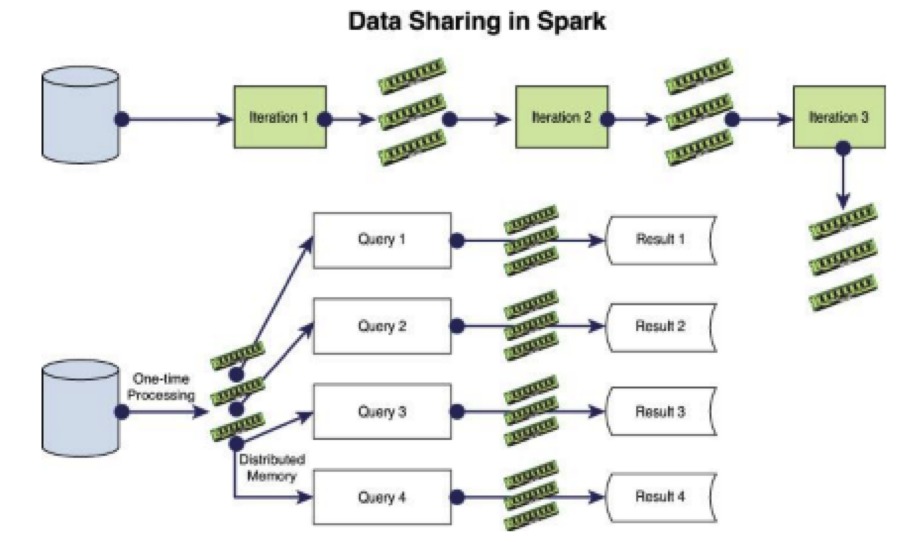
\includegraphics[width=1.0\textwidth]{bilder/3_spark.png}
\caption{Schematische Darstellung der Funktionsweise von Spark [VA14]}
\label{fig:sparkfunkt}
\end{figure}
  
\section{Das Konzept der RDD}
\label{section:rdd}



Bei den Resilient Distributed Datasets (RDD) in Spark handelt es sich um verteilte Objekt-Collections, die im Allgemeinen im Speicher der Cluster-Knoten gecached  und zwischen den Knoten bewegt werden. Sie können durch verschiedenste parallele Operatoren manipuliert und im Fehlerfall automatisch neu aufgebaut werden. Deshalb merken sich die RDDs die Transformationen, die zu ihrem Aufbau geführt haben und können so verlorene Daten schnell rekonstruieren. Da es sich bei RDDs prinzipiell um Scala-Collections handelt, können diese auch direkt in Scala-Code eingebunden und verarbeitet werden, oder interaktiv über die Scala-Konsole REPL genutzt werden. RDDs können nur durch 




grobgranulare, deterministische Transformationen, wie beispielsweise map, filter, join, etc. erstellt werden. 

RDDs können prinzipiell auf drei Arten gespeichert werden [SP14]:
\begin{itemize}
		\item Als deserialisiertes Java-Objekt im Speicher der JVM – dieses Variante bietet die beste Performance, da die Objekte sich direkt im JVM-Heap befinden
		\item Als serialisiertes Java-Objekt direkt im Speicher – dieses Verfahren ist speicher-effizienter, aber schlechter in der Zugriffsgeschwindigkeit
		\item Im Dateisystem – diese Variante ist erwartungsgemäß die langsamste, jedoch nötig, wenn die RDDs zu groß für die Haltung im RAM sind. 		
\end{itemize}	





\section{Spark im Cluster}
\label{section:spark im cluster}


Spark-Anwendungen laufen als unabhängiges Set von Prozessen auf Cluster-Infrastrukturen. Das Hauptprogramm (Driver-Program) enthält das SparkContext-Objekt, das die einzelnen Prozesse koordiniert. Auf Clustersystemen hält der SparkContext die Verbindung zum jeweiligen Cluster-Manager (Mesos, Yarn), im Standalone-Betrieb instanziert der Context selbst einen Dummy-Manager und allokiert in beiden Fällen die für die Anwendung nötigen Hardware-Ressourcen.    

\begin{figure}[htb!]
\centering
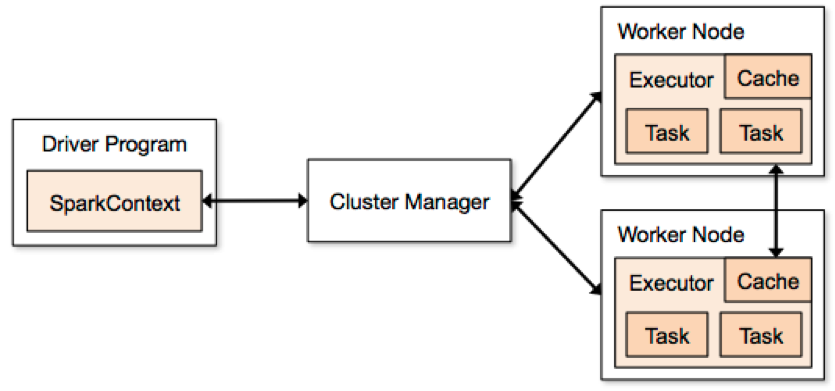
\includegraphics[width=1.0\textwidth]{bilder/3_2_cluster.png}
\caption{Clusteraufbau mit Spark [SP14]}
\label{fig:sparkcluster}
\end{figure} 






Wenn eine Verbindung aufgebaut ist, installiert Spark sogenannte Executors auf den Knoten des Clusters. Der Applikationscode wird nun als JAR direkt an die Executors geschickt und dieser anschließend durch entsprechende Tasks ausgeführt. 




































%%%%%%%%%%%%%%%%%%%%%%%%%%%%%%%%%%%%%%%%%%%%%%%%%%%%%%%%%%%%%%%
%% Verzeichnisse

\chapter{Verzeichnisse}
\label{chapter:verzeichnisse}
%\addcontentsline{toc}{chapter}{Verzeichnisse}

\bibliographystylelit{geralpha}
\bibliographylit{literaturVerzeichnis}
\addcontentsline{toc}{section}{Literaturverzeichnis}

%\newpage
\bibliographystyleint{geralpha}
\bibliographyint{internetQuellen}
\addcontentsline{toc}{section}{Internetquellen}

%\newpage
\listoffigures
\addcontentsline{toc}{section}{Abbildungsverzeichnis}
\clearpage
\cleardoublepage
%\newpage
\listoftables
\addcontentsline{toc}{section}{Tabellenverzeichnis}
\clearpage
\cleardoublepage
\lstlistoflistings 
\addcontentsline{toc}{section}{Quellenverzeichnis}
\clearpage
\cleardoublepage

%%%%%%%%%%%%%%%%%%%%%%%%%%%%%%%%%%%%%%%%%%%%%%%%%%%%%%%%%%%%%%%
%% Anhang

\clearpage\newpage
\begin{appendix}
  %%
%% Beuth Hochschule für Technik --  Abschlussarbeit
%%
%% Anhang
%%
%%%%%%%%%%%%%%%%%%%%%%%%%%%%%%%%%%%%%%%%%%%%%%%%%%%%%%%%%%%%%%%%%%%%%

\chapter{Zusätze}
\label{chapter:anhang}

\setglossarysection{section}
\printglossary[type=\acronymtype,title=Abkürzungen]


\section{Quelltext}
\label{section:quelltext}



\end{appendix}



\end{document}
